\subsection{Basics of MATLAB - Palm - Chapter 1}

\begin{enumerate}

\item \textbf{MATLAB(Current Directory, Workspace, Command Window, File)
interface}

When you double click MATLAB you will have a number of windows
present. The configuration of all windows in your MATLAB version may
be different but the names are all the same.

\begin{figure}[htb]
  \begin{center}
    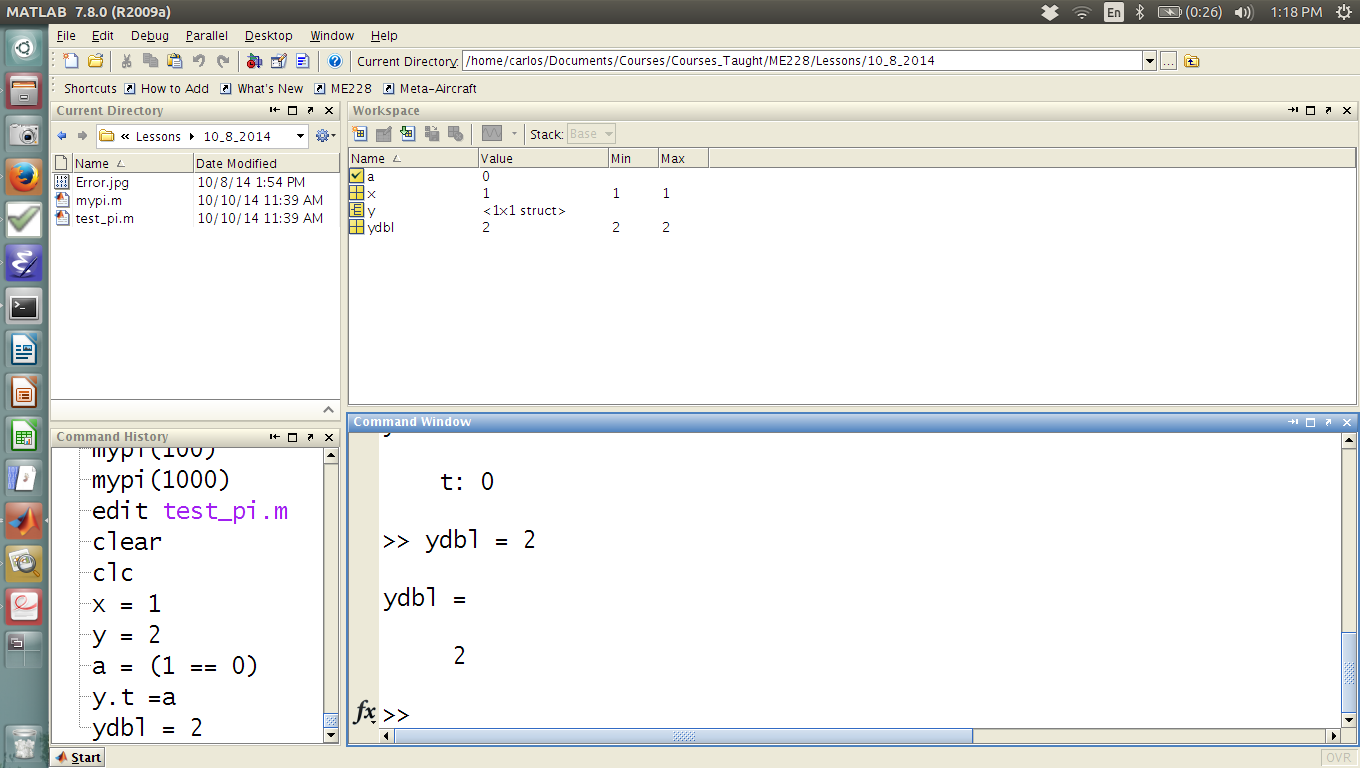
\includegraphics[height=0.55\textwidth,width=0.8\textwidth]{Graphics/MATLAB}
  \end{center}
\end{figure}

The very top of the MATLAB window is our toolbar. It has similar
buttons such as File, Edit, etc. Below this is your current
directory. This lists the current folder that you are operating
in. The window in the upper right is the Current Directory as well
which lists all the files currently in the folder. In this example I
have an error.jpg file, a mypi.m and test\_pi.m file. Note that a .jpg
is a picture file and a .m file is a MATLAB script file. The window
directly to the right is the Workspace. This lists all the current
variables in the workspace. The lower left window is my Command
History. It contains the history of all of my inputs into the Command
Window. The command window is where I can use MATLAB like a
calculator. If I type the following command

$>>$ x = 1

into the command window, MATLAB will create a variable 1 and save it
into x. Everytime I type in x it will now use 1 as the value. Thus, if
I type in 

$>>$ y = 2*x

the variable y will be evaluated as 2*x where x = 1 thus 2*1 = 2 and y
will be 2.

\item \textbf{Order of operations}

MATLAB works just like your calculator does. Thus, you need to make
sure parentheses are in the correct spot. For example

$>>$ x = 1/(2+1) 

will set x = to one third. However, 

$>>$ x = 1/2+1

will set x = 0.5 + 1 = 1.5. Try this in MATLAB to see the
difference. It is important to remember PEMDAS (Parentheses,
Exponents,Multiplication/Division, Addition/Substraction) That is,
MATLAB evaluates those operators in that order.

\item \textbf{Learn format of output}

There may be times when you need to see more than 4 significant
digits. For example,

$>>$ x = sqrt(2)

will output x = 1.4142. However it may be beneifical to see more
significant digits. To do that simply type

$>>$ format long g

into MATLAB. Then when you type 'x' into MATLAB you should see 13
digits. To return to normal output simply type

$>>$ format short g

\item \textbf{ What variables do I have?}

Sometime through your coding you will have alot of variables in your
workspace. For example it you type

$>>$ x = 2

$>>$ y = 2*x

$>>$ z = x\textrm{\^}2

In order to see all of your variables you can simply type 

$>>$ whos

into MATLAB. This will output all variable names in your workspace,
their size, the number of bytes they are taking up and the class which
is also known as type. Another way to see the current variables is to
simply look at the workspace window.

\item \textbf{ Variable Types}

There are numerous types of variables that MATLAB can handle. Think of
them as different currencies. For example I could give you a number
which is known as a double

$>>$ x = 42

or I could give you a set of characters known as a char.

$>>$ s = 'Hello World'

If I then type in 

$>>$ whos 

into MATLAB I see that I have a variable x with a size of 1x1, using 8
bytes, and a class of double. I also will have a variable s with a
size of 1x11, and a class of char. The size of s is 1x11 because I
have 11 characters in the variable. The space is included. The number
of bytes is equal to 2*11 or 22. That is because MATLAB needs 2 bytes
for every letter and thus needs 22 bytes to represent that number. A
double always needs 8 bytes. That is, the number 42 needs 8 bytes, the
number 6789 needs 8 bytes. The name double comes from the fact that
numbers are converted to binary which is of base 2. If I wish to
convert variables from one type to another I use the functions num2str
and str2num. 

$>>$ x = 1

$>>$ y = num2str(x)

The code above will convert the variable x to a string and save it in
y. Note that if you type whos into MATLAB x will still be a double but
y will be a string. Try using str2num to see what happens.

Note that the reason why MATLAB uses 2 bytes per character is because
it uses the unicode UTF-16 standard. Remember that 2 bytes is 16 bits
hence UTF-16. How many characters can UTF-16 represent? Check out the
entire list here.

http://www.fileformat.info/info/charset/UTF-16/list.htm

Obviously there are other formats such as UTF-7 and UTF-8 which stand
for 7 and 8 bit respectively. They all have their strengths and
weaknesses. 

\item \textbf{Scripting}

Alot of times you will have to compute something such as the number of
seconds in a day. This can be easily accomplished by typing.

$>>$ seconds\_min = 60

$>>$ seconds\_hour = 60*seconds\_min

$>>$ seconds\_day = 24*seconds\_hour

However, if you make a mistake you will have to clear everything

$>>$ clear

and start over. This can be very tedious. Thus scripting was
invented. 

\begin{enumerate}

\item \textbf{ Open a File...}

To open a file you can simply click File $\rightarrow$ New
$\rightarrow$ Blank M-File. Once the file is open you must save the
file by clicking File $\rightarrow$ Save. You can also type

$>>$ edit filename.m

into MATLAB and it will create a file called filename.m. If you then
return to the MATLAB window notice that you will have the file
filename.m in your current directory. If you type

$>>$ ls

into MATLAB you should also see your filename displayed there as
well. With the script open you can then create a script.

\item \textbf{Example Script}

Below is a simple script calculating the number of seconds in a
day. The first three lines clears the workspace, the command window
and closes all open figures. Note that the \% is a comment that can be
used to make notes in your script.

\begin{framed}

clear 

clc

close all

\%\%\%This is a comment

seconds\_min = 60

seconds\_hour = 60*seconds\_min

seconds\_day = 24*seconds\_hour

\end{framed}

\item \textbf{ Execute Script}

There are three ways to execute a script. 

\begin{enumerate}
  
\item Hit the play button from the top of the editor
\item Hit F5 on the keyboard
\item Type 

$>>$ filename 

in the command window. When you type filename in the command window,
MATLAB will search for a file called filename.m and execute the
contents of the script. If the file does not exist, MATLAB will throw
an error.

\end{enumerate}

\end{enumerate}

\item \textbf{Directories}

Further along you may download a file from the internet and open it in
MATLAB. When you do this the file will be opened in a editor in
MATLAB. However, when you attempt to run this script, MATLAB will ask
you whether or not you would like to change the current directory. If
you do this the current directory at the top toolbar will change to
the location of the file you just downloaded. Note that if you then
run another file you will have to change the directory again. I urge
you to try and organize your files such that everything makes
intuitive sense.

\item \textbf{Help!}

If at any point you ever lose your way simply type 

$>>$ help 

into MATLAB. If you know of a function but you forget what it does or
how to use it simply type

$>>$ help $<$variable name$>$

for example

$>>$ help num2str

will list what num2str does and how to use it.

\item {\bf Functions Learned}

whos

clear

clc

format long g

ls

num2str, str2num

disp

\end{enumerate}


